\setchapterpreamble[u]{\margintoc}
\chapter{Scenario Assessments}
\labch{scenario_assessments}

In this chapter I will go over the physical limitations of 100\% Renewable scenarios, from pumped storage locations and scale to batteries materials mining and photovoltaic and wind land area constraints.


\section{Pumped Storage Locations}

Let us try and see the scale needed to meet our energy capacity storage needs. In order to do that, we will look at a hypothetical facility, and then at what is being done today.

As we have discussed, pumped hydro storage is done by using the excess electricity we want to store to pump water up into a reservoir (lake). We can then get the electricity back similarly to a classical hydroelectric plant. The round-trip efficiency can be pretty high depending on the geographical characteristics.

We will now simplify matter and consider a pyramid shaped reservoir. This is not a correct way of representing a reservoir, but it is easy and a good approximation of the order of magnitude. We will consider that the wall is 500 meters high, the sides (valley width) are 2 kilometers apart, and the length (valley length used) 5 kilometers. The volume of water stored is then around 1.7 cubic kilometers\sidenote[][-2mm]{$V = \frac{1}{3}height * width * length$}. To account for the actual shape being a little larger due to the geometry approximation, let's assume that the reservoir clocks in at 2 cubic kilometers.

\begin{marginfigure}[-2mm]
	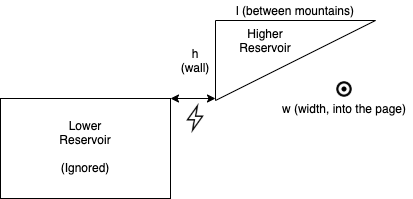
\includegraphics{schema_hydro}
	\caption[Quick schema of the pumped storage station]{Quick schema of the pumped storage station.}
	\labfig{schema_hydro}
\end{marginfigure}


\begin{remark}
Recall that to obtain the energy stored in our hypothetical facility, we simply have to use basic physics.

If $m$ is the mass of water in the reservoir, $g$ the gravitational acceleration constant and $h$ the height of the reservoir, then the potential energy stored in our reservoir is given by~\ref{potential_energy}\footnote{Mind the units!}.

\begin{equation}\label{potential_energy}
E = mgh
\end{equation}

For a 500 meters high wall, and the 2 cubic kilometer reservoir discussed in our hypothetical facility, we have a potential energy of

\begin{equation}\label{potential_energy}
E = 2 \times 10^9 * 1000 * 10 * 500 = 1 \times 10^{16} J = 2.8 TWh
\end{equation}

For a 300 meters high wall, the reservoir is now decreased to 1 cubic kilometer, say 1.2 cubic kilometer to account for the simplified geometry. This gives us 1 TWh.

\begin{equation}\label{potential_energy}
E = 1.2 \times 10^9 * 1000 * 10 * 300 = 1 TWh
\end{equation}

\end{remark}

To give a reference, the tallest dam in the world is 300 meters high. To meet the energy storage requirements of a France electricity grid in a 100\% renewable scenario, four of the giant dams should be built. And note that you need to find the location for it.

You can easily see that we are talking about an almost unimaginable scale. The largest dams in the world today would have to become among the smallest\sidenote[][-2mm]{There is a reason the tallest dam in the World, Itaipu Dam, is considered one of the seven wonders of the modern world}.

\begin{itemize}
\item Could every countries build one of these hypothetical facilities?
\end{itemize}

Some will say that it has been done before, so sure. But a lot of countries simply do not have favorable terrain.


\begin{itemize}
\item Could every countries build the necessary multiple infrastructure of this magnitude to meet their storage needs?
\end{itemize}

It is getting difficult to answer with nuance already. If it was the only goal of humanity, this could happen, I guess\ldots


\begin{itemize}
\item Could countries build all the world-record-breaking dams (along with the logistic of flooding valleys somehow) in less than a decade or two?
\end{itemize}

This one is a bit easier to answer. No.


Another things to keep in mind here is the sheer amount of concrete that would be necessary. The financial costs\sidenote[][-2mm]{An enterprise of this magnitude would profoundly change the markets} and, most importantly the energetic costs alone form a physical barrier that I personally cannot conceive being realistically overcome. The Three Gorges dam in China used 28 million cubic meters of concrete. At 700 kWh per cubic meters of concrete, we are talking about around 20 TWh of energy needed to build that structure simply for the concrete. And recall, we need several of those types of dams. It is also worth noting that the impact of concrete manufacturing on $\mathrm{CO_2}$ emissions is not negligible.

%(https://www.grida.no/resources/5404)

Appendix: gravity towers



\section{Materials I -- Lithium and Lead}

Let us consider batteries storage capacity now. We have seen in \refch{renewable_solution} what the batteries needs were for full-renewable scenarios for various countries.

Now, let us look at what this means in terms of feasibility. Batteries require materials, and it happens that the most used materials right now\sidenote[][-2mm]{And the main contributors to the falling costs} are Lithium-Ion batteries and Lead-Acid batteries. Both require, respectively and without surprise, Lithium and Lead, which are mined today. 

\begin{kaobox}[frametitle=The Most Important Question]
We have seen that the costs involved were a problem in and of themselves. But this does not mean this cannot be done, as it has been argued that it might not be that negative of an economic impact due to various, unpredictable factors. This begs the follow-up question:

\begin{itemize}
\item What is the scale of raw materials needed?
\end{itemize}

\end{kaobox}

We will first consider a simple world where Lithium-Ion batteries dominates the market due to prices, as seen today.

We have seen that on a first order, the USA alone would need to install at minima around 30TWh of energy storage capacity to transition its \emph{electric grid only} to a 100\% renewable scenario.

One needs around 130g of Lithium for each kWh delivered by a Li-Ion battery, or in other words, 0.13 MT of Lithium per TWh. Then, we can obtain the total amount of Lithium to be mined in order to install the battery systems needed\sidenote[][-2mm]{Once! Recall that the lifetime of a Li-Ion battery is between 10 to 15 years, which means that you need to mine new materials every time you want to replace your battery}. We see that in the case of the USA electric grid transition, one needs around 4 megatons of Lithium every 10 or so years. Over a century, this means close to 40 megatons. 

Here is the catch. The current proven reserves of Lithium in the world are estimated to be around 70MT.

This means that for the USA electrical grid only, I stress this, over 50\% of the total world reserve are needed. Keeping in mind that we want to transition the total energy production, and not only the electricity, that a few countries would want the Lithium for their own grids, and that Lithium is necessary in a lot of other devices today, we can easily see that this is not sustainable\sidenote[][-2mm]{Not to mention that I really doubt the costs of Lithium would not skyrocket given a supply scarcity, putting a full stop to the "Batteries will get cheaper" argument}.

Another interesting thing to note is that Lithium is not homogeneously distributed in the world, as shown on \vreffig{lithium_reserves_world}. Most of the reserves come from South America, and from mines that China recently invested a lot to buy out. This is not my field, but I would not be surprised if this caused some very strong political tensions in the near future.


\begin{figure*}[h]
	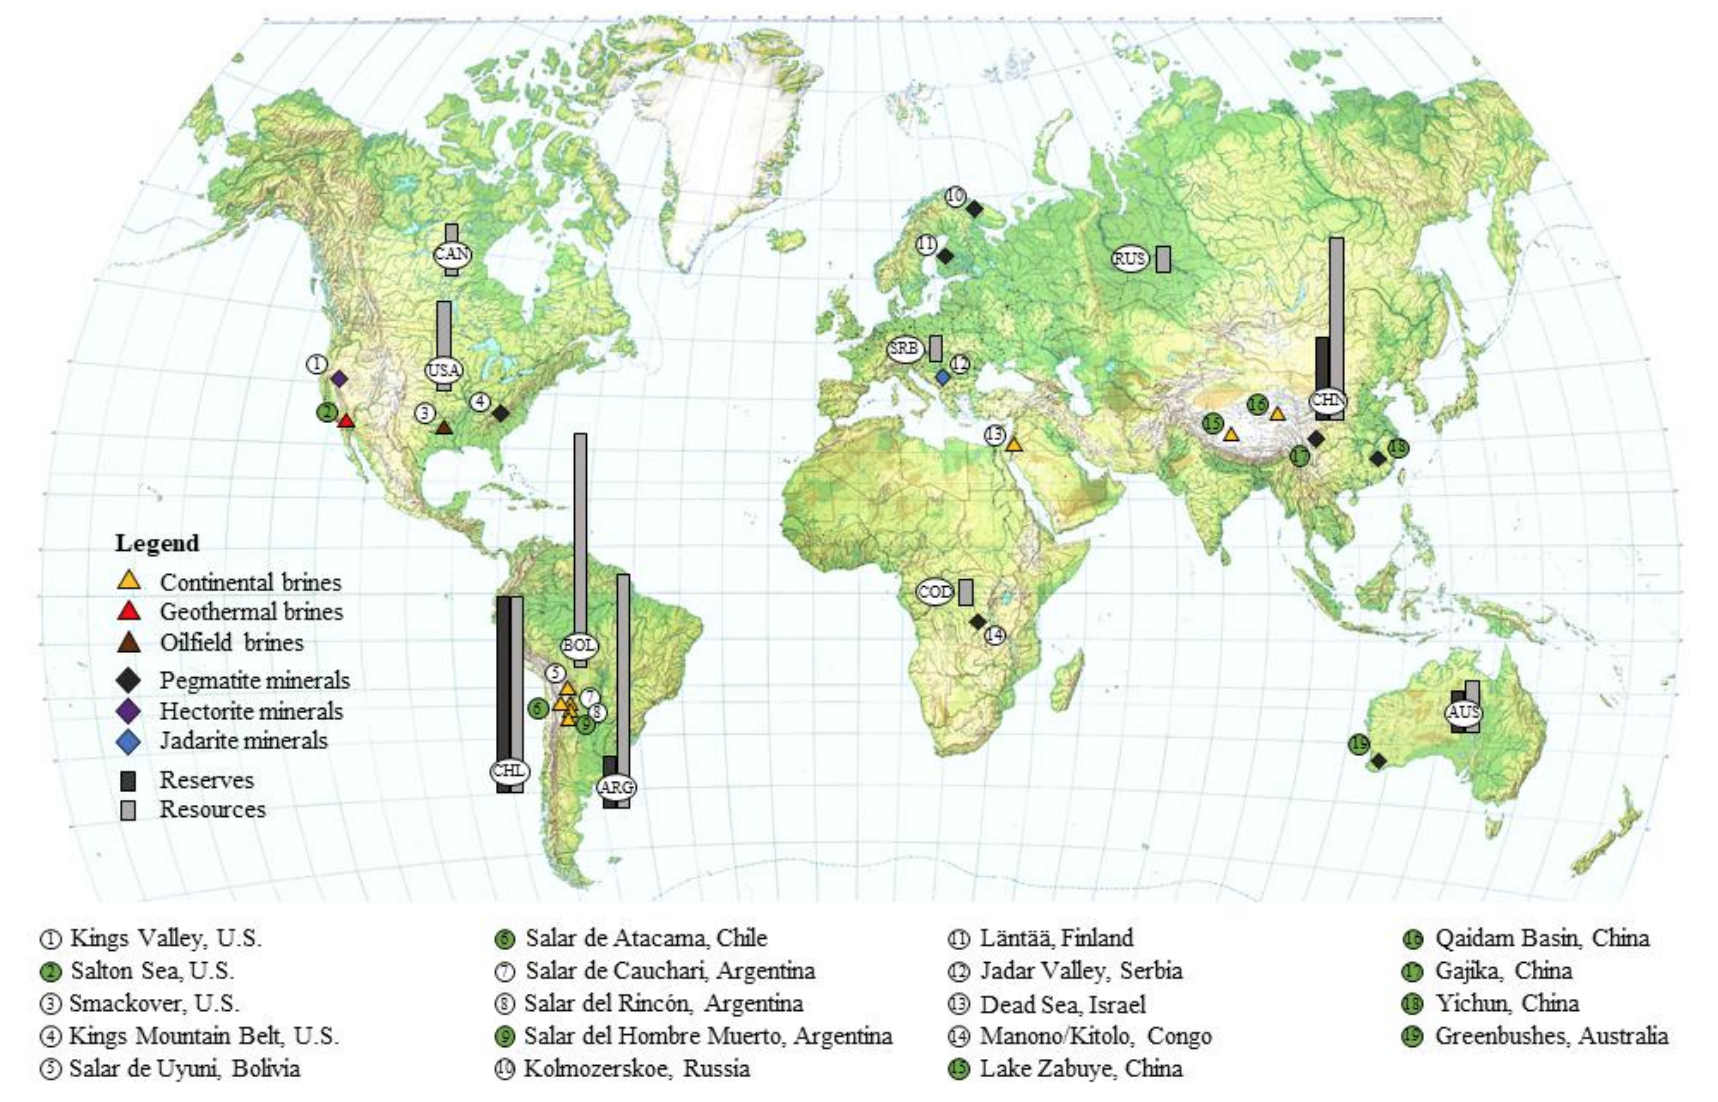
\includegraphics[width=1.0\textwidth]{lithium_reserves_world}
	\caption[Location of selected Li deposits and geographical distribution of global reserves and resources. Green colored labels are sites
known or believed to be currently producing.]{Location of selected Li deposits and geographical distribution of global reserves and resources. Green colored labels are sites
known or believed to be currently producing.}
	\labfig{lithium_reserves_world}
\end{figure*}

Let us take a look at the Lead-Acid batteries now, and do a similar assessment of their scaling potential. A Lead-Acid battery contains around 15 kg of Lead per kWh produced. Again, for the USA electrical grid transition, this amounts to 450 MT of Lead every 10 or so years, and 4,500 MT of Lead over the century.

Now, to the catch again. The proven resources of Lead in the world are around 80 MT, and the undiscovered resources estimated at around 2,000 MT. This is an obvious problem, as it is by far lower than the USA requirements to transition their grid alone.

Something to keep in mind in all this is that recycling is an option. Today, it is well developed for Lead, with around 50\% potentially recovered, putting the proven reserves at approximately 50\% more, up to 3,000 MT undiscovered. The recycling process for Lithium is more complex and is still under development\sidenote[][-2mm]{And considering the plastic recycling economy, I find it personally unlikely that this would make great strides necessary to have a scaling effect}. 

\section{Materials II -- Rare Earth Materials}


We saw the problem of Lithium and Lead. You may also have heard of the Rare Earth Elements problem.

\begin{kaobox}[frametitle=Rare Earth Materials]

Rare Earth Elements consists of seventeen metals, most of which are absolutely critical in numerous modern technologies. Yet they are difficult to extract from the crust.

Neodymium and Dysprosium are notably used extensively in wind turbine technology.

\end{kaobox}

We have estimated reserves of 8 MT of Neodymium and 1.5MT of Dysprosium in the world today. Wind power uses approximately 180 kg of Neodymium and 30 kg of Dysprosium per MW.

This implies that the hard limit on installed wind power is around 45,000 GW or 45 TW\sidenote[][-2mm]{This is ignoring the numerous other critical uses of Dysprosium and Neodymium}.

The installed wind power capacity necessary to power the entire US energy sector using wind would be around 8 TW. Given the lifetime of the wind turbine, this puts us at around 30 TW over a century. Obviously, in reality the need would be lower as the grid is not going to be powered by 100\% wind. But it does go to show that in a energy mix of say 50/50 between solar and wind, not even considering the batteries issues we discussed, the world decarbonized energy needs would likely be causing consequential resource issues from Neodynium and Dysprosium notably.

Will we develop a more efficient, more sustainable technology along the way? Maybe. But there is absolutely no guarantees of this\sidenote[][-2mm]{There have been, and still are, strong motivations to avoid the use of Rare Earth Elements, if only due to geopolitical reasons: most of the more easily accessible resources are in China. They have yet to come to something, fingers crossed}.

This is not a show-stopper by any means, but it is something to have in mind, and another hint at the best solution, a complete mix of low-carbon sources.

\section{Materials III -- Copper}

We can see the pattern here, the finite material problem is the crux of the renewable world. Another material of vital importance in the manufacturing of wind turbines, solar panels, and batteries\sidenote[][-2mm]{On top of plethora of essential everyday items} is copper. The reason it is so prevalent is because of its great efficiency at conducting electricity.

Solar energy uses approximately 5,000 tons of copper per GW installed, while wind power uses 2,000 tons of copper per GW installed. Recall from the previous section that switching the entire grid to wind energy would require around 30 TW over a century. This represents 60 megatons of copper, only for the USA. Considering solar energy requires even more, it is safe to assume that this would be close to a lower bound.

And here is the catch\ldots The identified reserves are 2100 MT, with an estimated 3600 MT that are undiscovered. The current annual demand for copper represents around 25 MT and accelerating quickly (0.5-1MT additional demand per year). 

\begin{lstlisting}[caption={An example of an incorrect interpolation.}]
year = 0
copper_consumption = 0  # MT
copper_reserves_estimated = 5700 # MT
rate_yearly_change = 0.5  # MT
while i < copper_reserves_estimated:
    copper_consumption += 25 * (1 + j*rate_yearly_change)
    year += 1
print(year)
\end{lstlisting}

Running this little code snippet shows that we can expect, under this rate increase and a business as usual scenario, that we would have around 30 years worth of reserves (identified and undiscovered).

We have discussed previously the danger of extrapolating into the future, and this is exactly what happened here. We took the rate of consumption increase and projected that ad infinitum. This is not a correct assumption, as it is obvious to see that the market would respond negatively to such a demand. In our case, with our simple first order approach, all we can really say is, well, nothing without a huge uncertainty range.

If we consider that demand stays constant, which is actually a fair, optimistic lower bound in today's digital world, then we see that we could get over two centuries of copper.

$\textrm{Years to depletion} = \frac{5700 \textrm{ (reserves)}}{25 \textrm{ (constant consumption)}} = 228 \textrm{ (years)}$

Or, another way to look at it is to consider what we are likely to use for our existing needs during the next century.

$5700\textrm{ (reserves) } - 100\textrm{ (years) } * 25\textrm{ (consumption) } = 3200\textrm{ (reserves left)}$

We can quickly identified that in this scenario, we will have consumed all the identified resources, and be left with the undiscovered resources\sidenote[][-2mm]{And they could be anywhere}, even before considering a real 100\% renewable worldwide push. Still, it is not unreasonable to assume that these resources can be discovered.

This seems pretty high. Now, let's apply a quick and dirty estimate of the world energy need in installed renewable capacity. The current energy consumption in the world is estimated at around 160000 TWh, or 160 PetaWh. From that let us compute the lower and higher bound of copper consumption from the energy transition to 100\% renewable.

Translating to wind power\sidenote[][-2mm]{recall that wind power has a lower copper usage than solar, and a higher capacity factor, so this would form a lower bound}, and assuming an average capacity factor of 30\%, we compute a needed installed capacity of around 60 TW. Given our time frame of a century for sustainability, we would need to install around 240 TW. At 2 megatons per TW, this brings us to 480 MT.

On the other hand, translating to solar power and assuming an average capacity factor of 20\%, we compute a needed installed capacity of around 
90 TW, or around 365 TW over a century. At 5 megatons per TW, this brings us to 1830 MT.

What we consequently see is that under a very favorable projected consumption rate, considered constant, the needs for Copper over the next century under a 100\% renewable scenario\sidenote[][-2mm]{Without accounting for batteries} can be grossly estimated between 3,000 and 4,300 megatons, or 52\% to 75\% of all undiscovered reserves, and 1.4 to 2 times the discovered resources.


\section{Locations I -- Renewable Siting}

\blindtext

\section{Health Production Impact}

Solar panel and intensive mining does cause a lot of problems today. This would need to be monitored for such a large extension

\blindtext



\section{The Digest}

\begin{kaoboxgreen}[frametitle=Main Takeaways]

\begin{itemize}
\item The \emph{finite materials problem} is very real and is an unmovable wall in the way of 100\% renewable scenarios.
\item Renewable energy is indeed renewable by definition, but capturing that energy is not renewable.
\item Building up energy storage systems or wind turbines use up either finite geographical locations or finite materials resources at an alarming and absolutely not sustainable rate.
\item Recycling will have to become prevalent for some materials. It will not be enough to cover the needs of a 100\% renewable system, but still absolutely needs to be developed.
\end{itemize}
  
\end{kaoboxgreen}